\documentclass[10pt,english]{beamer}
%\documentclass[english,handout]{beamer} % For handouts
\usetheme[progressbar=frametitle,block=fill]{metropolis} %numbering=none

%%% USEFUL PACKAGES
%\usepackage{showframe} % For debugging positioning
\usepackage{etex} % If too many packages
% Encoding and language
\usepackage[utf8]{inputenc}
\usepackage{babel}
\usepackage{amsmath, amssymb}
\usepackage{natbib}
%\usepackage{booktabs}
%\usepackage{algorithmic}
\usepackage{algorithm}
\usepackage{caption}
%\usepackage{animate} % Animations
\usepackage{bm} % Bold math
\usepackage{bbm}
%\usepackage{url}
%\usepackage{pifont}
%\usepackage{ulem} % Used for strikeouts \sout
%\usepackage{stackengine}
%\usepackage{enumitem}
%\setlist[description]{leftmargin=\parindent,labelindent=\parindent}
%\usepackage{colortbl} % Used for colored rows in tables


%%% GRAPHICS
\usepackage{graphicx}
\graphicspath{{./figs/}}


%%% COLORS
\setbeamercolor{background canvas}{bg=white}
\def\BlankFrame{
	\bgroup
	%\pdfpageheight 29.7cm
	\setbeamercolor{background canvas}{bg=}
	\begin{frame}[plain]
	\end{frame}
	%\makeatletter
	%\pdfpageheight \beamer@paperheight
	%\makeatother
	\egroup}

\usepackage{xcolor}
\definecolor{DarkGreen}{HTML}{00B200}
\definecolor{LightBlue}{HTML}{0090D9}
\definecolor{gold}{rgb}{.812,.710,.231}
% Text markup
%\setbeamercolor{alerted text}{fg=red}
\newcommand{\blue}[1]{\textcolor{blue}{#1}}
\newcommand{\red}[1]{\textcolor{red}{#1}}
\newcommand{\grey}[1]{\textcolor{gray}{#1}}
\newcommand{\orange}[1]{\textcolor{mLightBrown}{#1}}
\newcommand\myheading[1]{\textbf{#1}}
\newcommand\myemph[1]{\underline{\emph{#1}}}
\newcommand\textexample[1]{\textit{\textbf{#1}}}

%%% SPACING
\newcommand\vws[1][1]{\vspace{#1\baselineskip}} % vertical white space
%\newcommand\strt[1][1.5ex]{\rule[-.05\baselineskip]{0pt}{#1}} % strut
\newcommand\strt[2]{\rule[-#1ex]{0pt}{#2ex}} % strut
\newcommand\Hrule{\vspace{1ex} \hrule \vspace{1ex}} % Horisontal rule with some space after

%%% MISC
\newcommand\articleref[4]{\noindent\begin{minipage}[t]{0.04\textwidth}
		\vspace{0pt} 
		\pgfuseimage{beamericonarticle}
	\end{minipage}%
	\begin{minipage}[t]{0.96\textwidth}
		\vspace{0pt}
		#1. \textbf{#2.} \textit{#3}, #4.
	\end{minipage}}

%%% METROPOLIS THEME SPECIFIC
\makeatletter
\setlength{\metropolis@progressonsectionpage@linewidth}{1pt}
\makeatother
%\setbeamercolor{progress bar}{fg=red,bg=red!50}


%%% TEXTPOS
\usepackage[absolute,overlay]{textpos} % option showboxes is useful in draft mode
\setlength{\TPHorizModule}{\paperwidth}
\setlength{\TPVertModule}{\paperheight}
\textblockorigin{0pt}{10mm} % start everything at top-left, below gray 


%%% TIKZ/PGFPLOTS
\usepackage{tikz}
\usetikzlibrary{arrows,positioning,calc,shapes.geometric}
%\usetikzlibrary{arrows,calc,shapes.geometric,decorations.pathmorphing,backgrounds,positioning,fit,petri,decorations.pathreplacing}
%\usepackage{pgfplots}
%\pgfplotsset{compat = 1.3}


%%% BLOCKS AND BOXES
% Changing colors of blocks
%\setbeamercolor{block title alerted}{bg=UURed,fg=palette primary.fg}
%\setbeamercolor{block body alerted}{bg=UURed!15}
\setbeamercolor{block title alerted}{bg=mLightBrown,fg=palette primary.fg}
\setbeamercolor{block body alerted}{bg=mLightBrown!15}
%\setbeamercolor{block title example}{bg=UUGreen,fg=palette primary.fg}
%\setbeamercolor{block body example}{bg=UUGreen!10}
% \mybox is a rectangular box
\usepackage{boxedminipage}
\setlength\fboxrule{2pt}
\setlength\fboxsep{2\fboxsep}
\newcommand\mybox[3][\textwidth]{
  {\color{#2}
    \begin{boxedminipage}{#1}
      {\color{palette primary.bg} #3}
    \end{boxedminipage}}%
}   
\usepackage{tcolorbox}
\tcbset{arc=1mm,grow to left by=3mm,grow to right by=3mm,left=2mm}
%\newenvironment{redbox}{%
%	\begin{tcolorbox}[colback=UURed!15,colframe=UURed]}{%
%	\end{tcolorbox}}
%\newenvironment{greenbox}{%
%	\begin{tcolorbox}[colback=UUGreen!15,colframe=UUGreen]}{%
%	\end{tcolorbox}}
\newenvironment{redbox}{%
	\begin{tcolorbox}[colback=red!15,colframe=red]}{%
	\end{tcolorbox}}
\newenvironment{greenbox}{%
	\begin{tcolorbox}[colback=DarkGreen!15,colframe=DarkGreen]}{%
	\end{tcolorbox}}
\newenvironment{graybox}{%
	\begin{tcolorbox}[colback=mDarkTeal!5,colframe=mDarkTeal]}{%
	\end{tcolorbox}}
\newenvironment{orangebox}{%
\begin{tcolorbox}[colback=mLightBrown!15,colframe=mLightBrown]}{%
	\end{tcolorbox}}
\newenvironment{bwbox}{%
	\begin{tcolorbox}[colback=white,colframe=black]}{%
\end{tcolorbox}}
\newenvironment{bluebox}{%
	\begin{tcolorbox}[colback=LightBlue!15,colframe=LightBlue]}{%
\end{tcolorbox}}


%%%%%%%%% NEW MACROS

\newcommand\imp[1]{\alert{\textbf{#1}}}
\newcommand\bfit[1]{\textbf{\textit{#1}}}
\newcommand\good{\color{DarkGreen}{$\blacktriangle$}} % used in lists
\newcommand\bad{\color{red}{$\blacktriangledown$}} % used in lists


\RequirePackage{amsmath, amssymb}
\RequirePackage{bbm}
%\RequirePackage{newtxmath}


% Convenience macro for referring to data source
\newcommand\sourceurl[2]{\small \grey{Data from \href{#1}{#2}}}

% Abbreviations
\RequirePackage{xspace}
\newcommand\pdf{pdf\xspace}
\newcommand\ifft{iff\xspace}
\newcommand\ex{\textbf{ex)}\xspace}

% General time series notation
\newcommand\T{n}  % Length of time series
\newcommand\rtheta{{\red{\theta}}}  % Parameter (color coded)
\newcommand\rthetah{{\red{\widehat\theta}}}  % Estimate (color coded)

% Neural netowkrs
\newcommand\h{\mathbf{h}} % Hidden state variable
\newcommand\zz{\mathbf{z}} % Generic input (vector)

% For OLS/AR
\newcommand\noise{\varepsilon}  % This is the noise in AR, but should it be the same as measurement noise in SSM?
\newcommand\noisevar{\sigma^2_\noise}
\newcommand\noisevarhat{\widehat\sigma^2_\noise}
\newcommand\X{\Phi}
\newcommand\y{\mathbf{y}}
\newcommand\bphi{\bm\phi}

% State space models
\newcommand\z{\alpha}  % State vector, general SSM
\newcommand{\obsnoise}{\varepsilon}
\newcommand{\statenoise}{\eta}
\newcommand{\varobs}{\sigma^2_{\varepsilon}}
\newcommand{\varstate}{\sigma^2_{\eta}}
% For structural time series
\newcommand{\trendnoise}{\zeta}
\newcommand{\seasnoise}{\omega}
\newcommand{\vartrend}{\sigma^2_{\trendnoise}}
\newcommand{\varseas}{\sigma^2_{\seasnoise}}

%
\newcommand\FF{T}
\newcommand\GG{R}
\newcommand\HH{Z}
\newcommand{\covobs}{\sigma_\epsilon^2}
\newcommand{\covstate}{Q}
\newcommand\initmean{a_1}
\newcommand\initcov{P_1}
% Kalman filter
\newcommand{\zpart}[2]{\z_{#1}^{#2}}
\newcommand{\wgt}[2]{\omega_{#1}^{#2}}
\newcommand{\wgtsum}[1]{\Omega_{#1}}
\newcommand\zhat[2]{\hat\z_{#1|#2}}
\newcommand\Phat[2]{P_{#1|#2}}
\newcommand\zpred[1]{\zhat{#1}{#1-1}}
\newcommand\Ppred[1]{\Phat{#1}{#1-1}}
\newcommand\zfilt[1]{\zhat{#1}{#1}}
\newcommand\Pfilt[1]{\Phat{#1}{#1}}
\newcommand\ypred[1]{\hat y_{#1|#1-1}}
\newcommand\Spred[1]{F_{#1|#1-1}}
\newcommand\Spredinv[1]{\Spred{#1}^{-1}}
\newcommand\epshat[2]{\hat{\obsnoise}_{#1|#2}}
\newcommand\etahat[2]{\hat{\statenoise}_{#1|#2}}

\newcommand{\statefun}{T}
\newcommand{\obsfun}{Z}
\newcommand{\estfun}{h}

\newcommand{\qd}{q} %State density
\newcommand{\md}{g} %Measure density

\newcommand{\rmd}{\mathrm{d}}

% SMC
\newcommand{\Np}{N}           % Number of particles
\newcommand{\Mp}{M}           % Number of particles in backward simulation



%\RequirePackage{color}
%\newcommand{\flnote}[1]{{\color{red}\textbf{[#1]}}} % Used for notes in text - color red
%\newcommand\Hrule{\vspace{1ex} \hrule \vspace{1ex}} % Horisontal rule with some space after; This is moved to beamer preamble

%%%%%%%%%%%%%%%%%%%%%%%%%%%%%%%%%%%%%%%%%%%%%%%%%%%%%%%%%%%%%%%%%%%%%%%%%%%%%%%%
%                            COMMANDS IN TEXT                                  %
%%%%%%%%%%%%%%%%%%%%%%%%%%%%%%%%%%%%%%%%%%%%%%%%%%%%%%%%%%%%%%%%%%%%%%%%%%%%%%%%
\newcommand\numtext[2]{#1\textsuperscript{#2}}
\newcommand\thsnd[1]{\ensuremath{#1\thinspace000}}
\newcommand{\peqref}[1]{\eqref{#1} on page~\pageref{#1}} % Page referencing for equations: "(1) on page 1"

%%%%%%%%%%%%%%%%%%%%%%%%%%%%%%%%%%%%%%%%%%%%%%%%%%%%%%%%%%%%%%%%%%%%%%%%%%%%%%%%
%                            SPECIFIC MATH                                     %
%%%%%%%%%%%%%%%%%%%%%%%%%%%%%%%%%%%%%%%%%%%%%%%%%%%%%%%%%%%%%%%%%%%%%%%%%%%%%%%%
% Models etc.
%\newcommand{\T}{T}            % Number of samples in data record
\newcommand{\parspace}{\Theta}                                   % Parameter space
\newcommand{\parameter}{\theta}                                  % Parameter
% Spaces
\newcommand{\setX}{\ensuremath{\mathsf{X}}}                      % State-space X
\newcommand{\sigmaX}{\ensuremath{\mathcal{X}}}                   % Sigma algebra on X
\newcommand{\setY}{\ensuremath{\mathsf{Y}}}                      % State-space Y
\newcommand{\sigmaY}{\ensuremath{\mathcal{Y}}}                   % Sigma algebra on Y
\newcommand{\setZ}{\ensuremath{\mathsf{Z}}}                      % State-space Z
\newcommand{\sigmaZ}{\ensuremath{\mathcal{Z}}}                   % Sigma algebra on Z

%%%%%%%%%%%%%%%%%%%%%%%%%%%%%%%%%%%%%%%%%%%%%%%%%%%%%%%%%%%%%%%%%%%%%%%%%%%%%%%%
%                           GENERAL MATH                                       %
%%%%%%%%%%%%%%%%%%%%%%%%%%%%%%%%%%%%%%%%%%%%%%%%%%%%%%%%%%%%%%%%%%%%%%%%%%%%%%%%

% ======== Miscellaneous symbols ========
\newcommand\eqdef{:=}
\newcommand\defeq{=:}
\newcommand\const{\text{const.}}
%\newcommand\eqdef{\stackrel{\text{\scriptsize def}}{=}}

\newcommand\iid{iid}
\newcommand{\iidsim}{\stackrel{\text{\iid}}{\sim}} % iid simulation
\newcommand{\process}[1]{\{#1\}_{t\geq 1}}       % Process (time index t)
\newcommand{\range}[2]{#1, \, \dots, \, #2}      % Range = 1, ..., N
\newcommand{\crange}[2]{\{#1, \, \dots, \, #2\}} % Curly range = {1, ..., N}
\newcommand{\prange}[2]{(#1, \, \dots, \, #2)}   % Parenthesised range = (1, ..., N)
\newcommand{\bwdrange}[2]{#1 : -1 : #2}          % Range = N, ..., 1
\newcommand{\approxpropto}{\stackrel{\sim}\propto}

% Tight dots between \int and \int in a multidimensional integral
\newcommand{\tightcdots}{\hspace*{-0.38em}\cdot\hspace*{-0.3em}\cdot\hspace*{-0.3em}\cdot\hspace*{-0.38em}}

% Arrows - convergence and mappings
% \mapsto                                                     % Mappings, x \mapsto f(x)
\newcommand{\fromto}{\rightarrow}                             % Mapping from set A to set B; f: A \fromto B
\newcommand{\goesto}{\rightarrow}                             % limits used in n \goesto \infty
\newcommand{\goestosmall}{\to}                                % limits used in \lim_{n \goestosmall \infty}
\newcommand{\convP}{\stackrel{\probab}\longrightarrow}        % Convergence in probability
\newcommand{\convD}{\stackrel{\textrm{D}}\longrightarrow}     % Convergence in distribution

% ======== Standard spaces  ========
\newcommand{\naturals}{\ensuremath{\mathbb{N}}}               % Natural numbers
\newcommand{\reals}{\ensuremath{\mathbb{R}}}                  % Real numbers
\newcommand{\nonnegatives}{\reals_{\smaller +}}               % Nonnegative numbers
\newcommand{\positives}{\reals_{\smaller ++}}                 % Positive numbers
\newcommand{\nonnegativedefinites}[1]{S_{\smaller +}(#1)}     % Nonnegative #1 x #1 matrices
\newcommand{\positivedefinites}[1]{S_{++}(#1)}                % Positive #1 x #1 matrices

% ======== Matrices ========
\newcommand{\eye}[1]{I_{#1}}                     % Identity matrix
\newcommand{\+}{\mathsf{T}}                      % Transpose
\newcommand{\kronecker}{\raisebox{1pt}{\ensuremath{\otimes}}} % Kronecker product
\DeclareMathOperator*\diag{diag}
\DeclareMathOperator*\trace{tr}

% ======== Operators, calculus etc. ========
\newcommand{\Ordo}{O}                            % Big ordo
\newcommand{\supnorm}[1]{\|#1\|_\infty}          % Supremum norm
\newcommand\osc{\text{osc}}                      % Oscillator norm
\newcommand{\grad}{\nabla}                       % Gradient
\newcommand{\complementof}[1]{\ensuremath{#1^\mathsf{c}}} % Set complement
\renewcommand\vec{\text{vec}}
\DeclareMathOperator*\supp{supp}                          % Support
\DeclareMathOperator*\card{card}                          % Set cardinality
\DeclareMathOperator*\rank{rank}                          % Rank
\DeclareMathOperator*\sign{sign}                          % Signum function
\DeclareMathOperator*\argmax{arg\,max}
\DeclareMathOperator*\argmin{arg\,min}

% ======== Probability ========
\newcommand{\Prb}{\ensuremath{\mathbb{P}}}                       % Probability
\newcommand{\E}{\ensuremath{\mathbb{E}}}                         % Expectation
\newcommand{\var}{\ensuremath{\mathrm{Var}}}                     % Variance
\newcommand{\cov}{\ensuremath{\mathrm{Cov}}}                     % Covariance
\newcommand{\cor}{\ensuremath{\mathrm{Corr}}}                     % Correlation
\newcommand{\I}{\ensuremath{\mathbbm{1}}}						 % Indicator function

%\newcommand{\abscont}{\ensuremath{\ll}}          % Absolute continuity
\renewcommand\mid{\,\vert\,} % I don't really like that \mid produces rubber lengths. Sometimes, we get very large white spaces p(x    |   y), and it can produce line breaks after "p(x |" . Is the non-rubber definition here better?
\newcommand\Mid{\,\middle\vert\,} % Stretchable |, to use with \left \right - N.B. This produces a longer | in general. Does that look better than a standard \mid?


% Distributions
\newcommand{\N}{\ensuremath{\mathcal{N}}}        % Normal
\newcommand{\uni}{\ensuremath{\mathcal{U}}}      % Uniform
\newcommand\MN{\mathcal{MN}}                     % Matrix normal
\newcommand\IW{\mathcal{IW}}                     % Inverse-Wishart
\newcommand\GP{\mathcal{GP}}                     % Gaussian process
\DeclareMathOperator*\Mult{Mult}                 % Multinomial
\DeclareMathOperator*\cat{Cat}                   % Categorical
\DeclareMathOperator*\Discrete{Discrete}         % Categorical/alternative name
\DeclareMathOperator*\bin{Bin}                   % Binomial
\DeclareMathOperator*\gam{Gam}                   % Gamma
\DeclareMathOperator*\St{St}                     % Student's t
\DeclareMathOperator*\po{Po}                   % Binomial

%\usepackage{extendedalt}
%\usepackage{animate} % Animations
%\usepackage{../lindsten}
%\usepackage{movie15}

\title{732G12 Data Mining}
\subtitle{Föreläsning 6}
\date{}
\author{Josef Wilzén \\ IDA, Linköping University, Sweden}
\titlegraphic{\hfill
\includegraphics[height=1.2cm]{../LiU_primary_black.pdf}}
%\institute{Joint work with\dots}


%% MY DEF %%
\newcommand{\itm}[1]{\mathrm{Item}_{#1}}
\newcommand{\pausa}{\pause}
%\renewcommand{\pausa}{}


\newenvironment{nscenter}
 {\parskip=0pt\par\nopagebreak\centering}
 {\par\noindent\ignorespacesafterend}

\begin{document}

\maketitle

\begin{frame}{Dagens föreläsning}

    \begin{itemize}
        \item Bayesianska klassificerare
        \item Ensamblemetoder
        \begin{itemize}
            \item Bagging
            \item Boosting
            \item Random forest
        \end{itemize}
    \end{itemize}
    
\end{frame}



\begin{frame}{Bayesiansk klassificerare}
    Att direkt modellera en icke-deterministisk funktion kan vara mycket svårt.

    Exempel:
    \begin{itemize}
        \item $(\text{diet}, \text{träning}) \to (\text{hjärtinfarkt})$ är svårt
        \item $(\text{diet}, \text{träning}) \to \mathbb{P}(\text{hjärtinfarkt})$ lättare
    \end{itemize}

    Använd Bayes sats för att hjälpa till i modelleringen
    \begin{align*}
        \mathbb{P}(Y \mid \mathbf{X}) &= \frac{\mathbb{P}(\mathbf{X} \mid Y)}{\mathbb{P}(\mathbf{X})} \cdot \mathbb{P}(Y) \propto \mathbb{P}(\mathbf{X} \mid Y) \cdot \mathbb{P}(Y) \\
        \text{posterior} &= \frac{\text{likelihood}}{\text{evidence}} \cdot \text{prior} \propto \text{likelihood} \cdot \text{prior}
    \end{align*}
\end{frame}

\begin{frame}{Kategoriska attribut}
    \begin{columns}
        \begin{column}{0.5\textwidth}
            $\mathbb{P}(Y = y)$ är andelen datapunkter med klass $y$.

            $\mathbb{P}(X_i = x_i \mid Y = y)$ andelen datapunkter med attribut $x_i$ av datapunkterna med klass $y$.
        \end{column}
        \begin{column}{0.5\textwidth}
            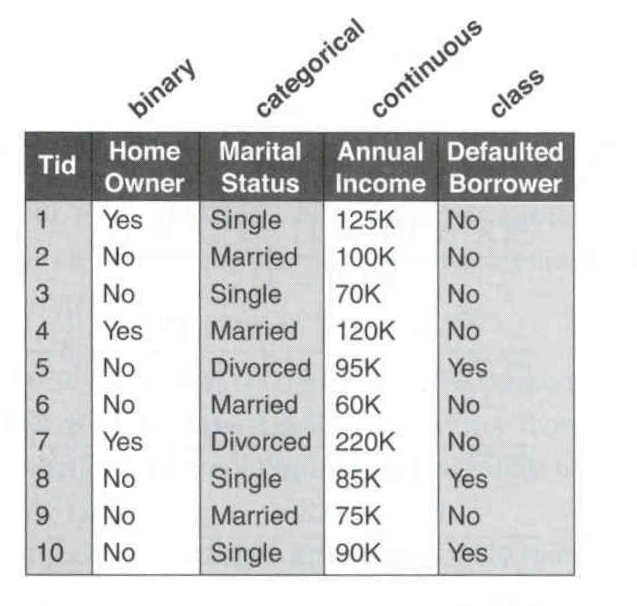
\includegraphics[width=\textwidth]{figs/data_bayes_class.png}
        \end{column}
    \end{columns}
\end{frame}

\begin{frame}{Kontinuerliga attribut}

    För kontinuerliga attribut finns olika tillvägagångssätt.

    \begin{itemize}
        \item Diskretisera data i olika kategorier.
        \begin{itemize}
            \item För få intervall gör att man missar information.
            \item För många intervall kan ge intervall utan observationer.
        \end{itemize}
        \item Anta en sannolikhetsfördelning för variabeln och skatta parametrarna från träniningsdatan.
        \begin{itemize}
            \item Normalfördelningen är vanlig.
            \item Conjugate prior.
        \end{itemize}
    \end{itemize}
    
\end{frame}

\begin{frame}{Grundläggande princip}

    Träningfasen:

    Skatta sannolikheten $\mathbb{P}(Y \mid \mathbf{X})$ för alla möjliga $\mathbf{X}$ och $y$.

    Klassificeringsfas:

    Givet $\mathbf{X}'$ skatta klass $Y' = \max_Y \mathbf{P}(Y \mid \mathbf{X}')$.
    
\end{frame}

\begin{frame}{Naiv Bayes klassificerare}

    Modellantagande:
    \begin{equation*}
        \mathbb{P}(\mathbf{X} \mid Y) = \prod_i \mathbb{P}(X_i \mid Y),
    \end{equation*}
    alla $X_i$ är oberoende av varandra. Vi kan då faktorisera likelihooden över $\mathbf{X}$.

    Använder vi detta får vi en sannolikhet
    \begin{equation*}
        \mathbb{P}(Y \mid \mathbf{X}) = \prod_i \mathbb{P}(X_i \mid Y) \mathbb{P}(Y),
    \end{equation*}
    det räcker med att skatta sannolikheten för varje $X_i$. Detta ger oss en enklare modell som går att skatta.
    
\end{frame}

\begin{frame}{Egenskaper hos naiv Bayes}
    \begin{itemize}
        \item Metoden är robust mot isolerade bruspunkter.
        \item Metoden är robust mot irrelevanta attribut.
        \item Lätt att skatta.
        \item Korrelerade attribut kan väsentligt försämra prestandan.
        \begin{itemize}
            \item Behöver en mer komplex modell för att hantera.
            \item Simultan sannolikhetsfördelning för likelihooden.
        \end{itemize}
    \end{itemize}
\end{frame}

\begin{frame}{Ensamblemetoder}
    
    Grundidén är att skatta många modeller på träningsdata och sen kombinera dessa för att göra prediktioner.
    
    Finns många olika varainter:
     \begin{itemize}
        \item Göra slumpmässiga urval från träningsdata och skatta modeller på dessa urval (Bootstraping/Bagging)
        \item Skapa en mängd dataset där observationerna har olika vikter i modellanpassningen i olika dataset (Boosting)
        \item Skatta ett antal olika modeller (kan vara av helt olika sort) och sen kombinera dessa vid prediktioner
        \item Vissa modeller har slumpmässiga element vid optimieringen (tänk neurala nätverk): optimera samma modell flera gånger men med olika seed, vilket ger olika modeller/parameterar. Kombinera dessa sedan vid prediktionen.
    \end{itemize}

\end{frame}


\begin{frame}{Ensamblemetoder}
    
    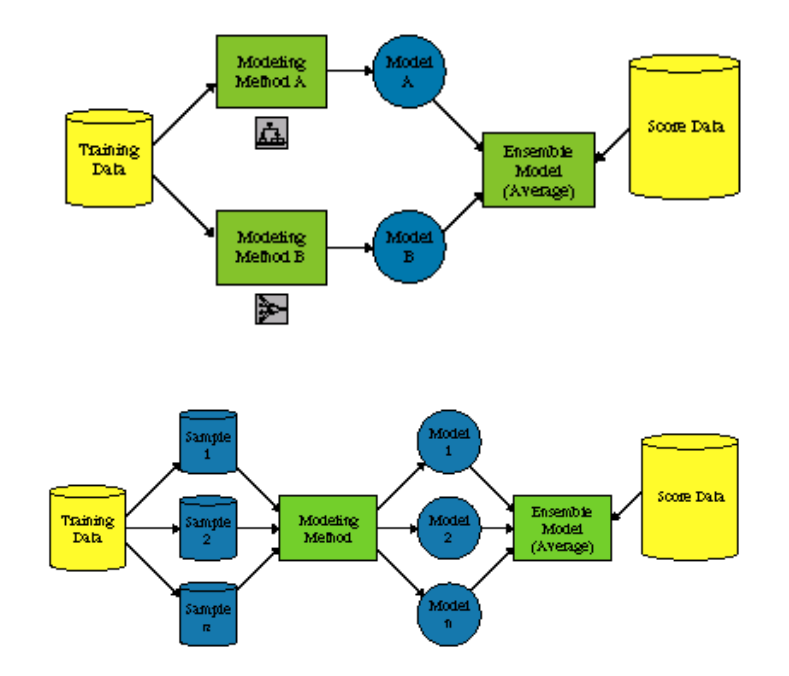
\includegraphics[width=.8\textwidth]{figs/ensample_cat.png}

\end{frame}

\begin{frame}{Bootstraping}
    
    \begin{greenbox}
        Idé: Skapa $B$ stickprov av datan genom att \textbf{med återläggning} välja nya datapunkter. Använd dessa stickprov för att skatta modell eller funktioner.
    \end{greenbox}

    Exempel:

    Vi vill skatta $\mathbb{V}(e^{\bar{X}})$.

    Skapa $B$ stickprov.

    Skatta $T_k = e^{\bar{Z}_k}$ för $k = 1, \ldots, B$.

    Beräkna $\mathbb{V}(\mathbf{T})$.


\end{frame}

\begin{frame}{Bagging}
    
    Idé: Om man tar medelvärdet av oberoende observationer (modeller) så minskar variansen.

    \begin{bluebox}
        \myheading{Bagging (Bootstrap aggregating)}: Använd Bootstrap för att skapa $B$ träningsdataset och skatta en modell $\hat{f}_b$ för varje av dessa set.

        Den slutgiltliga modellen får vi genom att ta medelvärdet av alla dessa modeller:
        \begin{equation*}
            \hat{f}_{\text{bag}}(\mathbf{X}) = \frac{1}{B}\sum_{b=1}^{B}\hat{f}_b(\mathbf{X}).
        \end{equation*}
    \end{bluebox}

    \begin{itemize}
        \item Sänker variansen av den anpassade funktionen.
        \item Påverkas \emph{mycket} av kvalitén av modellen. En bra modell blir bättre, en dålig blir sämre.
        \item För klassificering, använd majoritetsröstning.
    \end{itemize}

\end{frame}

\begin{frame}{Classification and Regression Trees (CART)}
    Vi delar upp variabelrummet genom att rekrusivt göra binära splittar.

    För klassificering används vanligaste klassen, för regression medelvärdet inom regionen.

    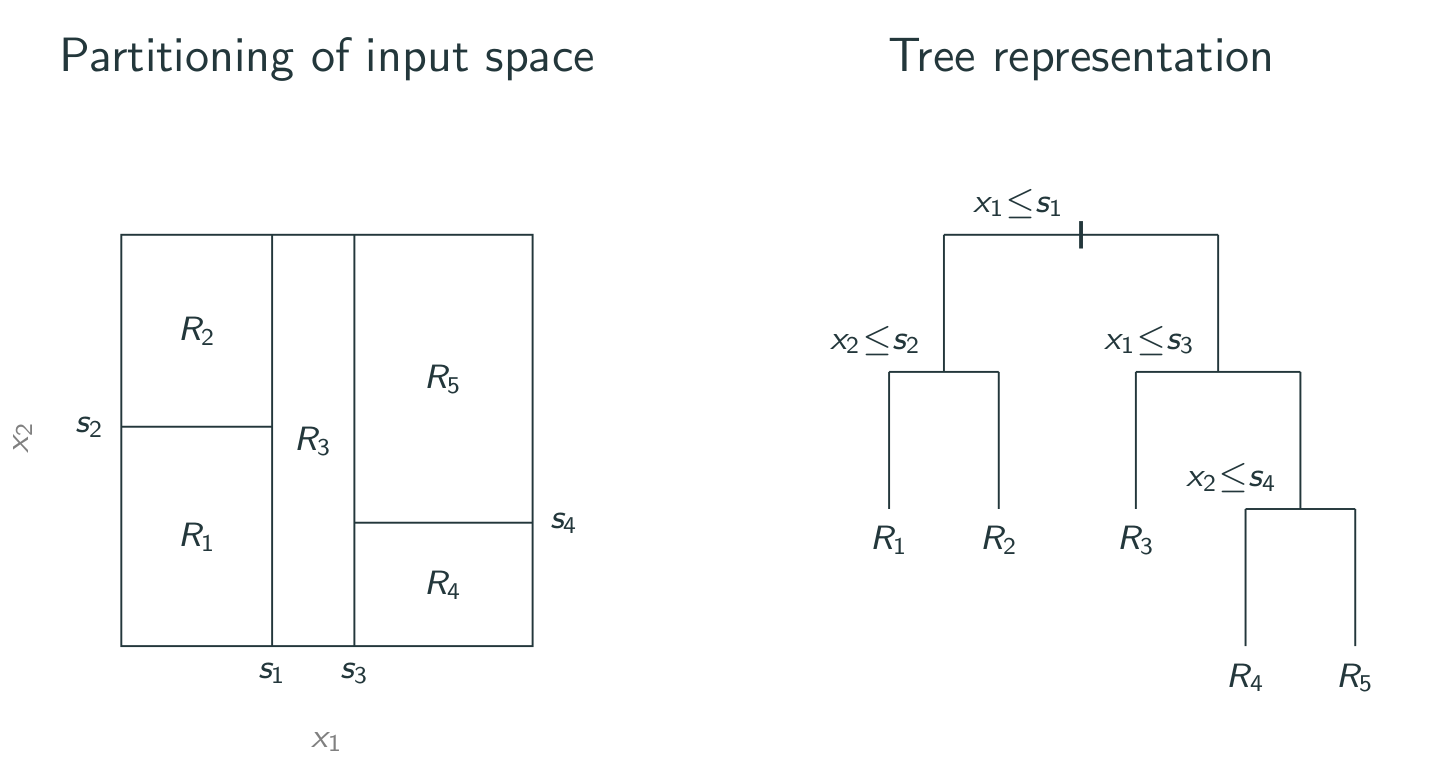
\includegraphics[width=0.8\textwidth]{figs/tree_fredrik.png}
\end{frame}

\begin{frame}{Förbättre CART}
    Flexibilitet/komplexitet för trädmodeller beror på djupet.
    \begin{redbox}
        Ett djupt träd ger litet bias, men mycket varians.
    \end{redbox}
    
    Förbättringar:
    \begin{itemize}
        \item Efterbeskärning (post-pruning):
        \begin{itemize}
            \item Skapa ett djupt träd och beskär det till ett mindre (minska variansen).
        \end{itemize}
        \item Ensamblemetoder:
        \begin{itemize}
            \item Ta ett genomsnitt över många trädmodeller.
            \item Bagging
            \item Random forest
            \item Boosted trees
        \end{itemize}
    \end{itemize}
\end{frame}

\begin{frame}{Random forest}
    
    Bagging kan ge stora förbättringar för trädmodeller. Men det finns vissa problem:
    \begin{itemize}
        \item De $B$ bootstrap-urvalen är korrelerade.
        \item Reduktionen i varians blir liten när vi tar medelvärde över korrelerade variabler.
    \end{itemize}

    Idé: Avkorrelera de $B$ trädmodellerna genom att göra slumpmässiga ändringar av modellerna.

\end{frame}

\begin{frame}{Random forest}
    
    \begin{itemize}
        \item Använd bagging för att skatta $B$ träd,
        \begin{itemize}
            \item Vid varje uppdelning/regel använd endast en slumpmässig delmängd $q \leq p$ av de förklarande variablerna.
        \end{itemize}
        \item Tumregel: (Förslag från Leo Breiman)
        \begin{itemize}
            \item Klassificering: $q = \sqrt{p}$
            \item Regression: $q = p/3$
        \end{itemize}
    \end{itemize}

\end{frame}

\begin{frame}{Random forest}
    Slumpmässigt val av variabler leder till:
    \begin{description}
        \item[-] Minskar bias, men ofta mycket långsamt.
        \item[-] Lägger till varians till varje träd.
        \item[+] Avkorrelerar träden.
    \end{description}
    Ofta dominerar den avkorrelerade effekten vilket leder till att MSE minskar på testdata.
\end{frame}

\begin{frame}{Random forest}
    Beräkningsmässiga fördelar:
    \begin{itemize}
        \item Lätt att parallellisera.
        \item $q <  p$ minskar kostanden för vaje regel/uppdelning.
        \item Inte så många hyperparametrar.
    \end{itemize}
\end{frame}

\begin{frame}{Boosting}
    
    En enkel modell kan vanligtvis fånga vissa aspekter av datan.

    Kan vi lära oss en stor mängd enkla modeller som var och en lär sig en liten del av datarelationen och sen kombinera dessa "dåliga" modeller till en stark modell.

    Hur skulle vi göra detta?

\end{frame}

\begin{frame}{Boosting}
    \begin{itemize}
        \item Lär sig sekventiellt en ensamble av "svaga" modeller.
        \item Kombinerar dessa till en "stark" modell.
        \item Generell metod som kan användas till all form av övervakad inlärning.
        \item Mycket framgångsrikt inom maskininlärning.
    \end{itemize}

    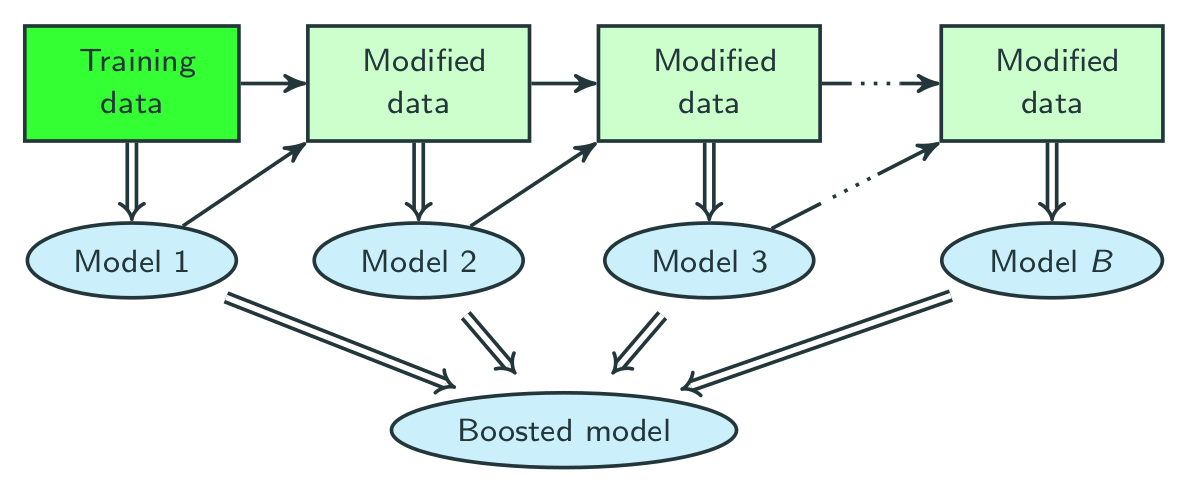
\includegraphics[width=\textwidth]{figs/boosting_scheme.png}
\end{frame}

\begin{frame}{Binär klassificering}
    Vi kommer begränsa oss nu till binär klassificering.

    Vi låter klasserna vara $-1$ och $1$ (möjliga $y$ värden).

    Använder vi detta kan vi skriva majoritetsröstninig av $B$ klassificerare $\hat{y}^{b}(\mathbf{x})$ som
    \begin{equation*}
        \sign \left(\sum_{b=1}^{B} \hat{y}^{b}(\mathbf{x})\right).
    \end{equation*}
\end{frame}

\begin{frame}{Boosting för klassificering}
    
    \begin{enumerate}
        \item Ge varje datapunkt en vikt $w_i^1 = 1/n$.
        \item För $b = 1, \ldots, B$
        \begin{enumerate}
            \item[a] Träna en "svag" klassificerare $\hat{y}^{b}(\mathbf{x})$ på den \myheading{viktade träniningsdatan} $\{(\mathbf{x}_i,y_i,w_i^b)\}_{i=1}^{n}$.
            \item[b] Uppdatera vikterna $\{w_{i}^{b+1}\}_{i=1}^{n}$ från $\{w_{i}^{b}\}_{i=1}^{n}$
            \begin{enumerate}
                \item[i] Öka vikterna för missklassificerade datapunkter.
                \item[ii] Minska vikterna för korrekt klassificeradet datapunkter. 
            \end{enumerate}
        \end{enumerate}
    \end{enumerate}

    Predikationen från de $B$ klassificerarna kombineras genom att använda en viktad majoritetsomröstning,
    \begin{equation*}
        \hat{y}^{B}_{\text{boost}}(\mathbf{x}) = \sign \left(\sum_{b=1}^{B} \alpha^b \hat{y}^b(\mathbf{x})\right).
    \end{equation*}

\end{frame}

\begin{frame}{Boosting exempel}
    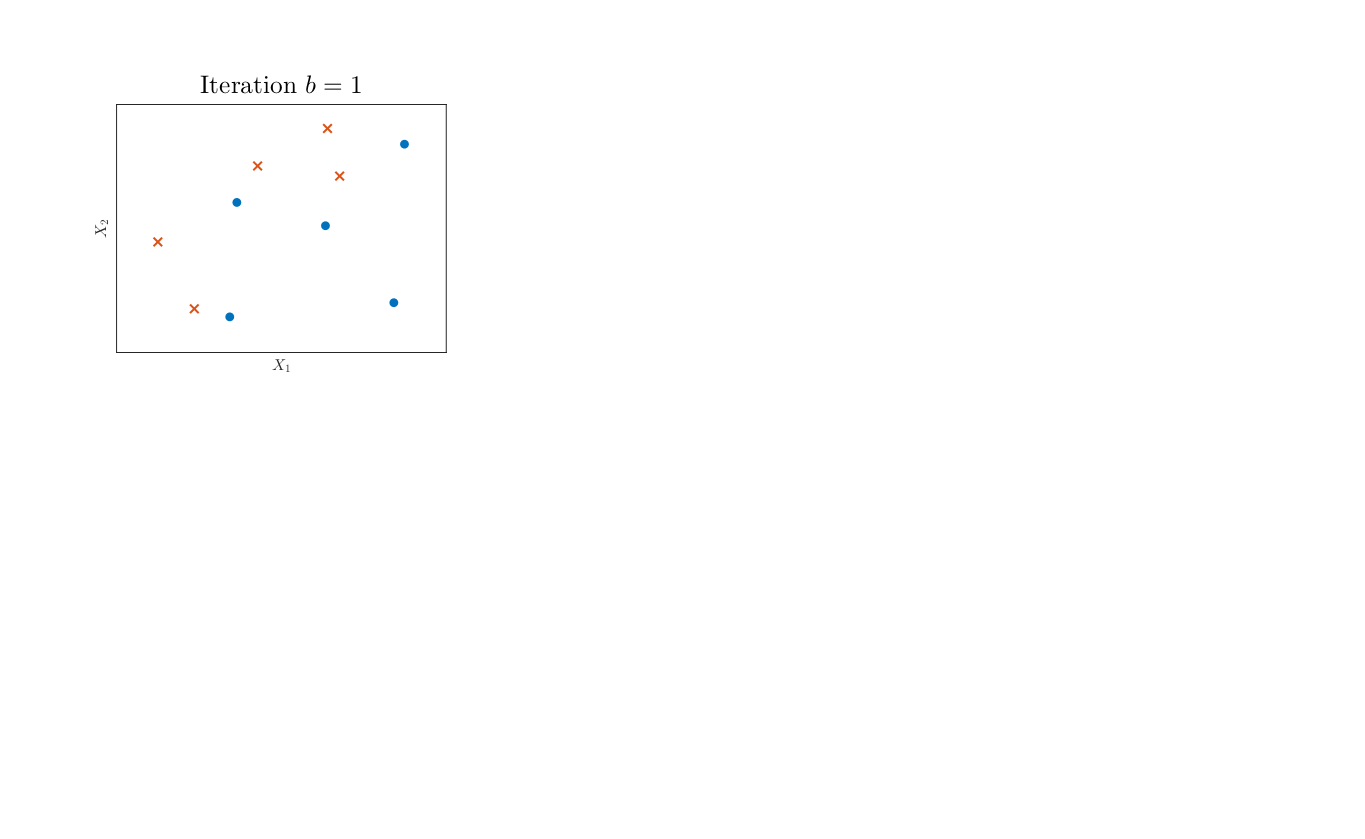
\includegraphics[width=\textwidth]{figs/Boosting illustration1.png}
\end{frame}

\begin{frame}{Boosting exempel}
    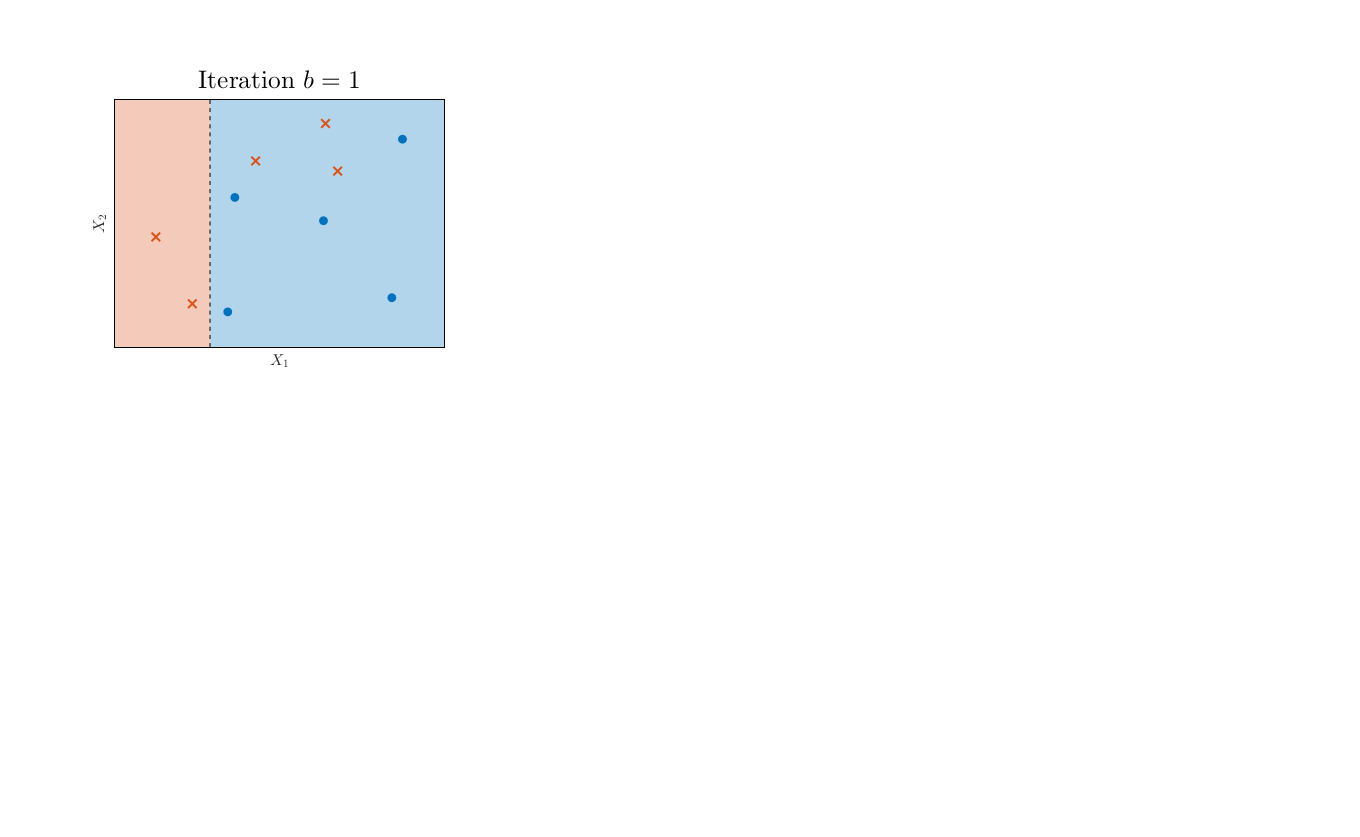
\includegraphics[width=\textwidth]{figs/Boosting illustration2.png}
\end{frame}

\begin{frame}{Boosting exempel}
    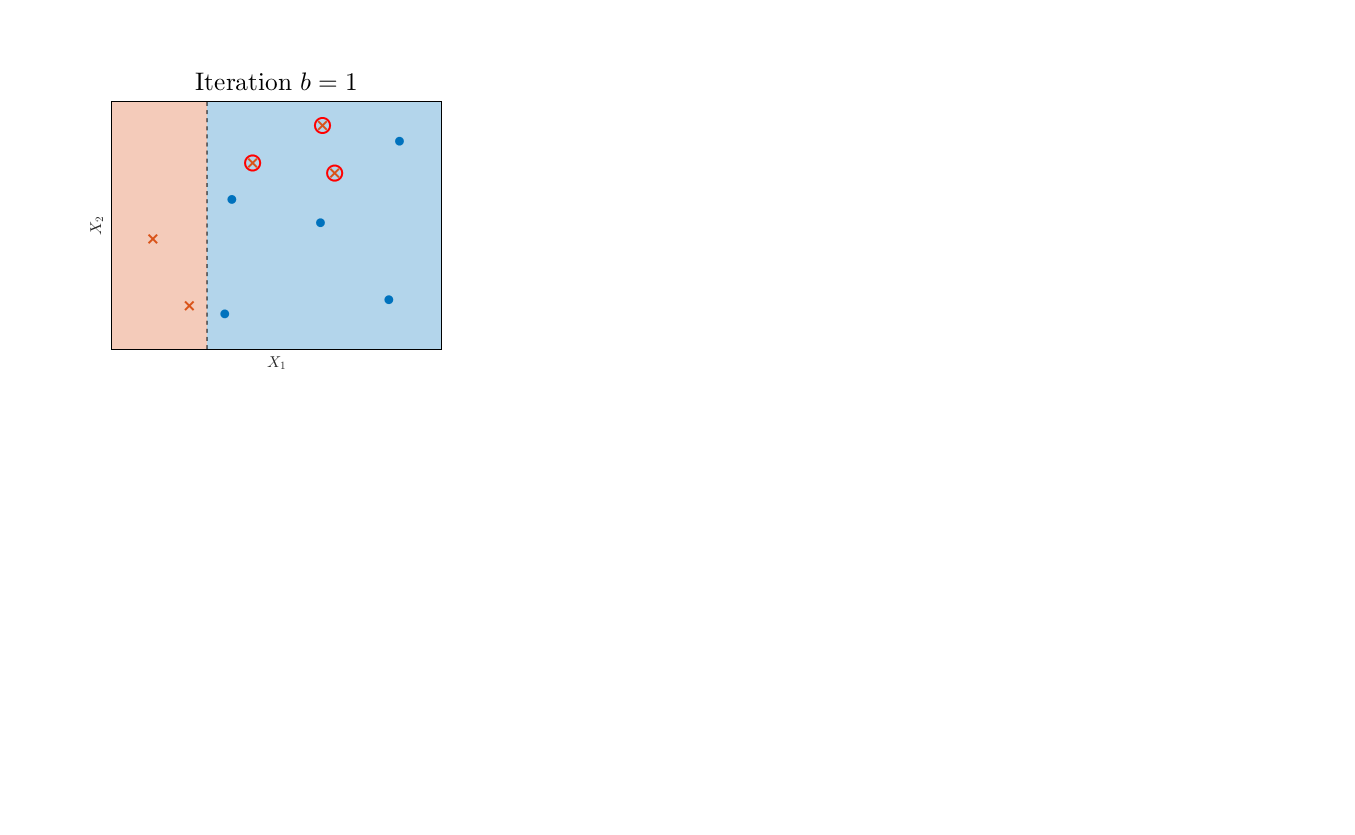
\includegraphics[width=\textwidth]{figs/Boosting illustration3.png}
\end{frame}

\begin{frame}{Boosting exempel}
    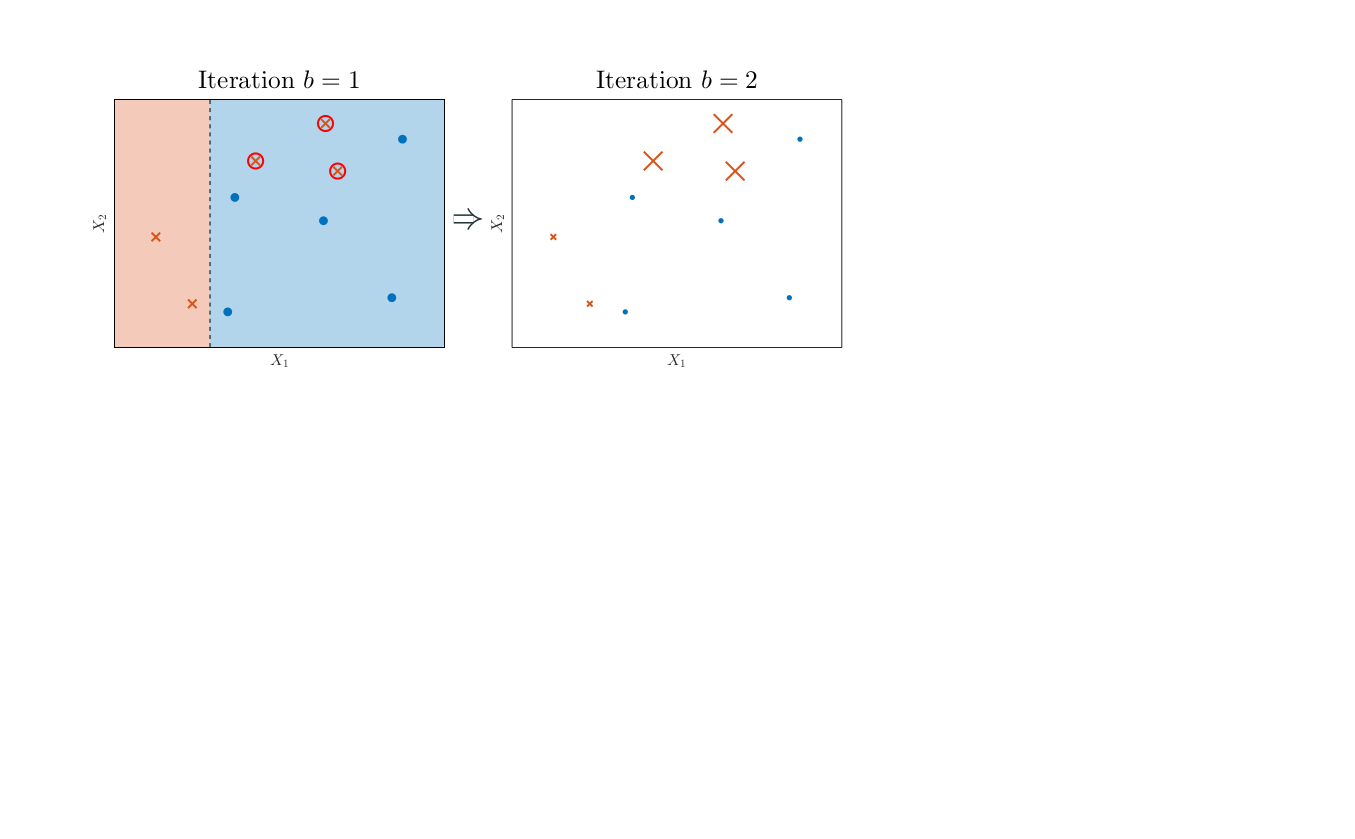
\includegraphics[width=\textwidth]{figs/Boosting illustration4.png}
\end{frame}

\begin{frame}{Boosting exempel}
    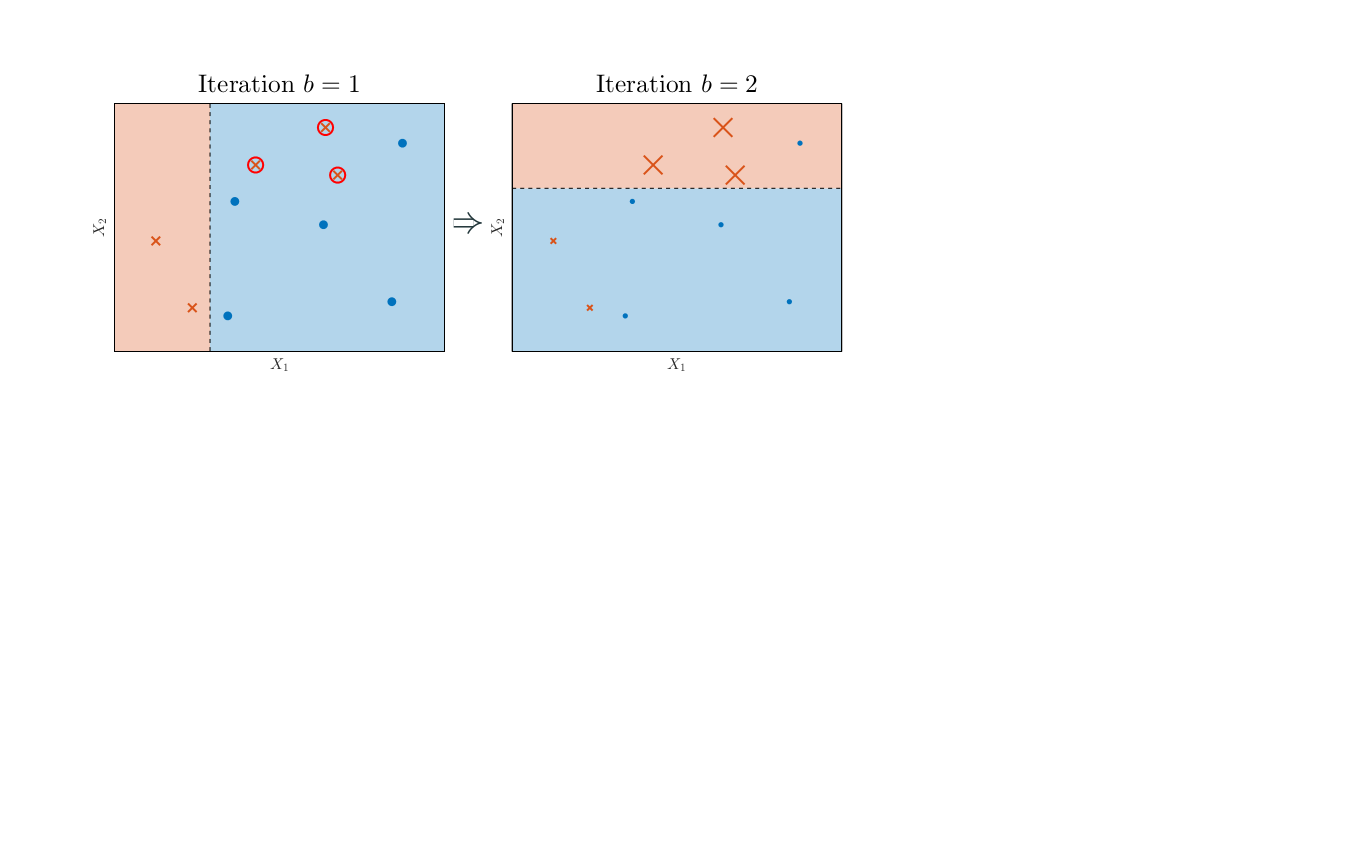
\includegraphics[width=\textwidth]{figs/Boosting illustration5.png}
\end{frame}

\begin{frame}{Boosting exempel}
    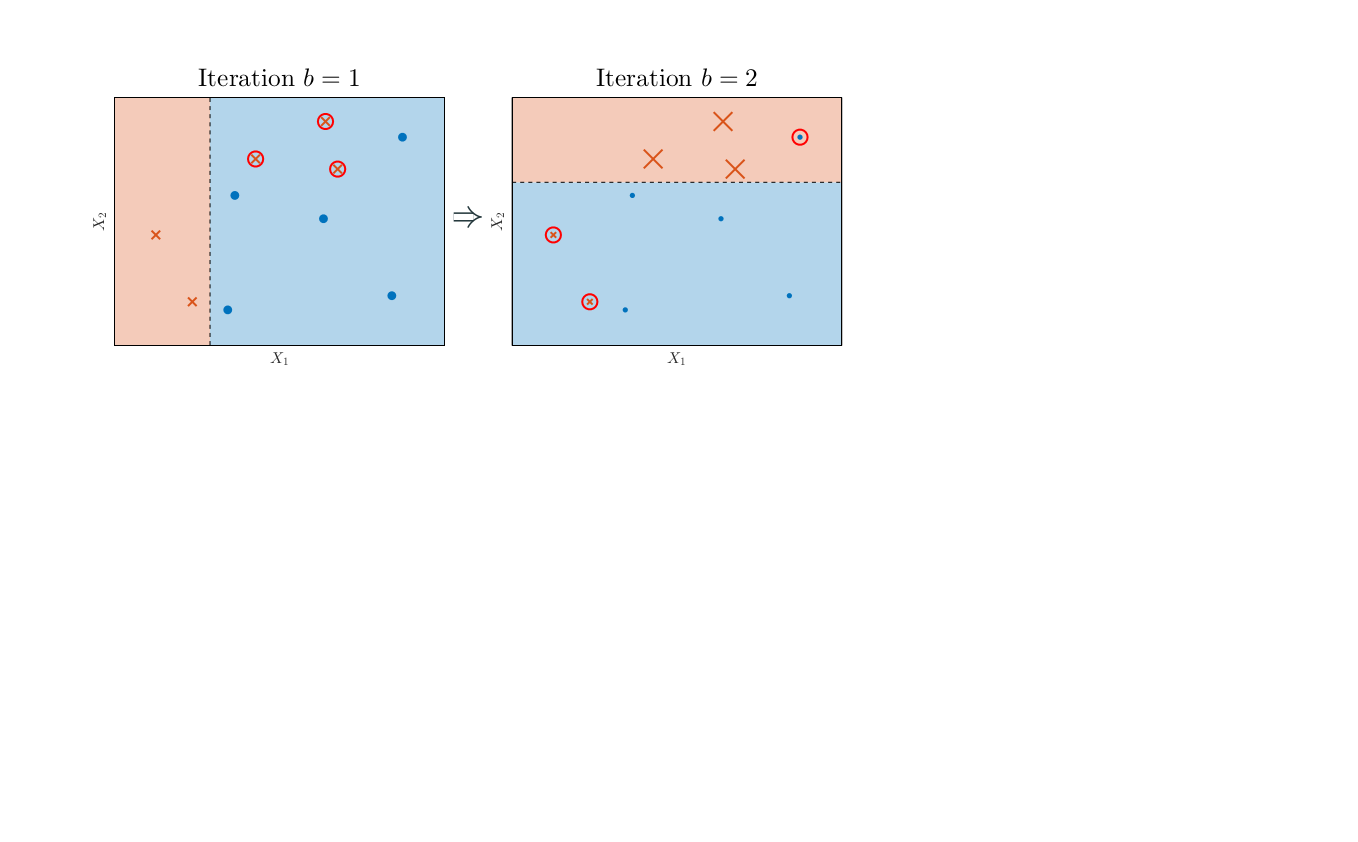
\includegraphics[width=\textwidth]{figs/Boosting illustration6.png}
\end{frame}

\begin{frame}{Boosting exempel}
    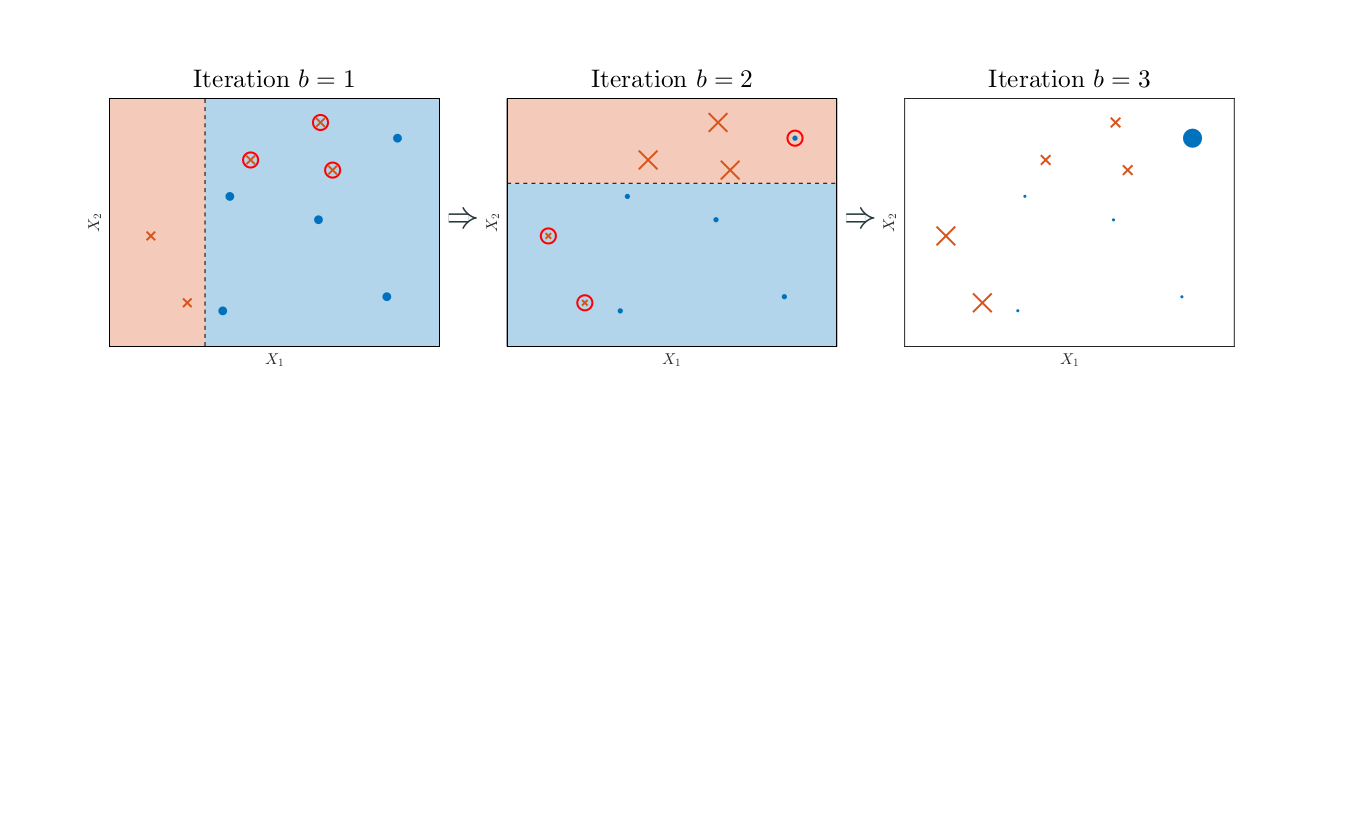
\includegraphics[width=\textwidth]{figs/Boosting illustration7.png}
\end{frame}

\begin{frame}{Boosting exempel}
    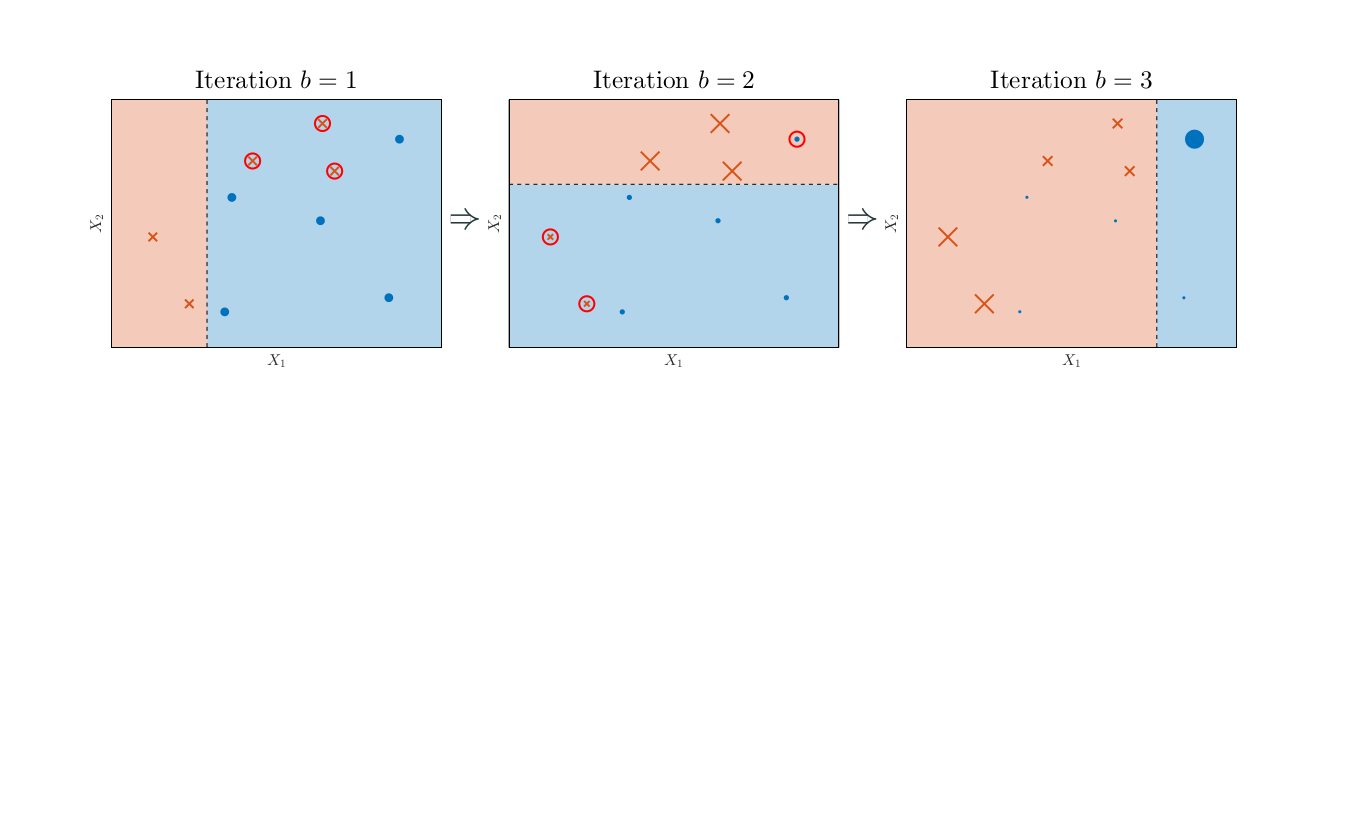
\includegraphics[width=\textwidth]{figs/Boosting illustration8.png}
\end{frame}

\begin{frame}{Boosting exempel}
    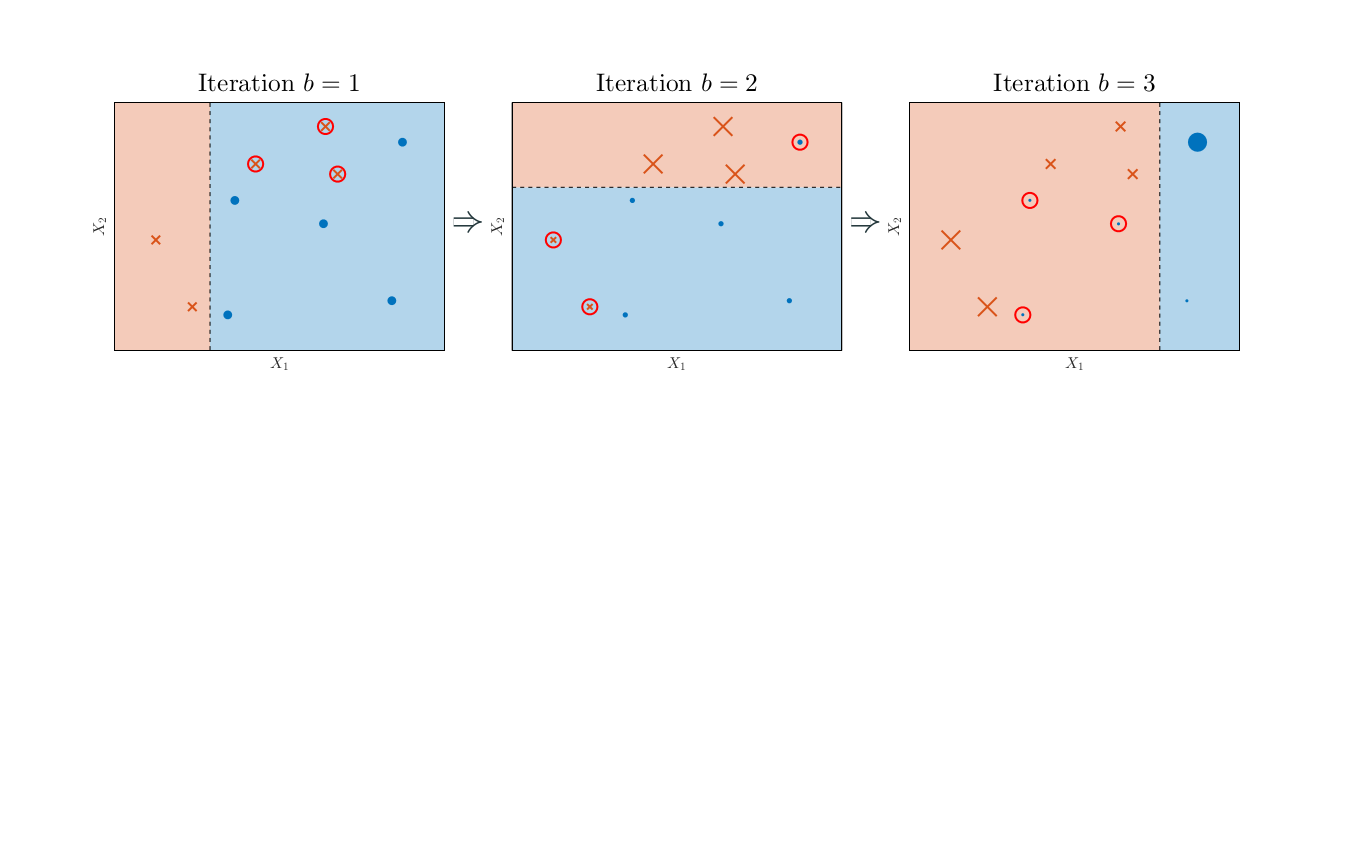
\includegraphics[width=\textwidth]{figs/Boosting illustration9.png}
\end{frame}

\begin{frame}{Boosting exempel}
    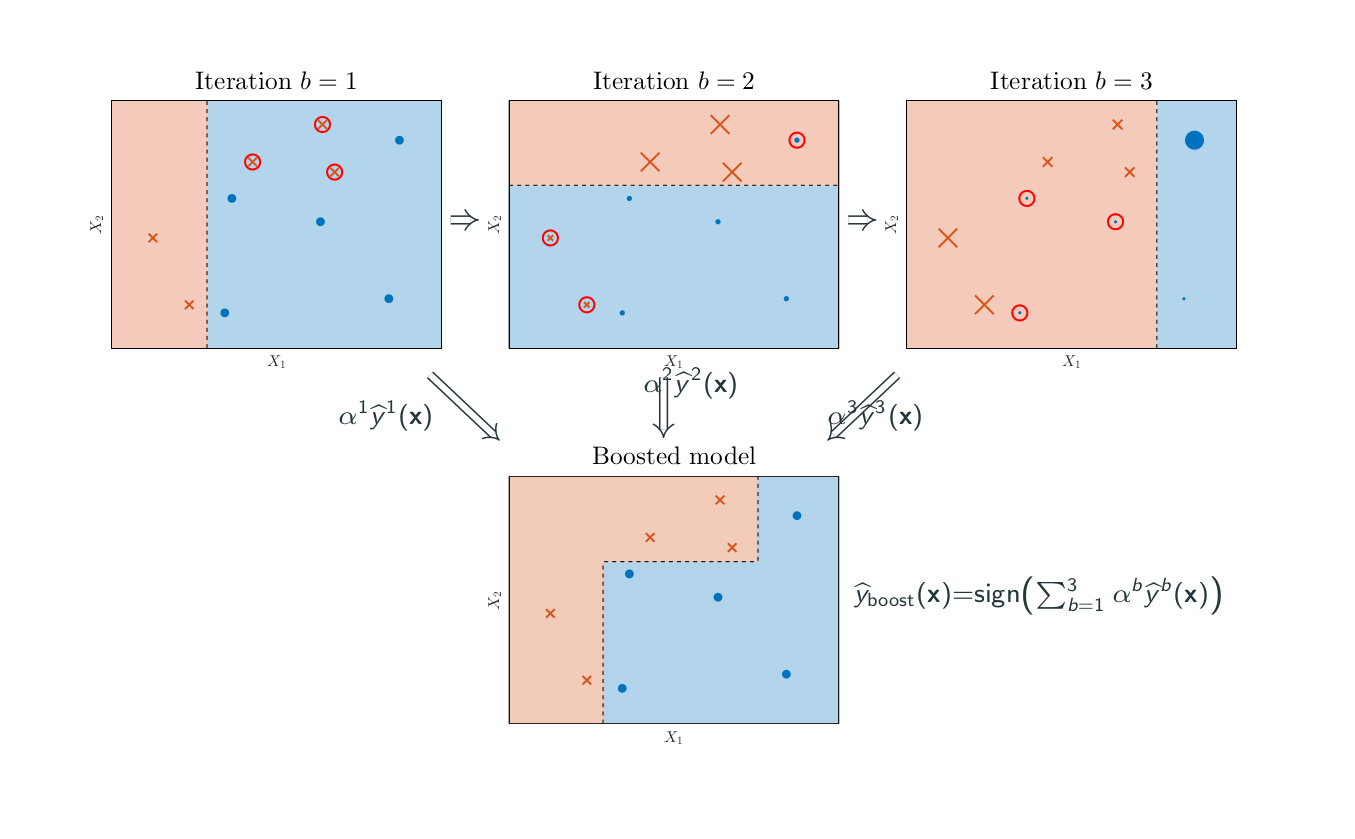
\includegraphics[width=\textwidth]{figs/Boosting illustration10.png}
\end{frame}

\begin{frame}{Boosting - Detaljer}
    
    Boosting fungerar bra, men vi har lite detaljer vi måste reda ut först.

    \begin{enumerate}
        \item Hur ska vi vikta om data?
        \item Hur ska vi vikta koefficienterna $\alpha^b$?
    \end{enumerate}

    Olika boostingalgoritmer svarar olika på dessa frågor.

    Den första praktiska algoritmen AdaBoost, svarade på dessa frågor genom att minimera exponentialförlust.

\end{frame}

\begin{frame}{AdaBoost}

    \begin{enumerate}
        \item Ge varje datapunkt en vikt $w_i^1 = 1/n$.
        \item För $b = 1, \ldots, B$
        \begin{enumerate}
            \item[a] Träna en "svag" klassificerare $\hat{y}^{b}(\mathbf{x})$ på den \myheading{viktade träniningsdatan} $\{(\mathbf{x}_i,y_i,w_i^b)\}_{i=1}^{n}$.
            \item[b] Uppdatera vikterna $\{w_{i}^{b+1}\}_{i=1}^{n}$ från $\{w_{i}^{b}\}_{i=1}^{n}$
            \begin{enumerate}
                \item[i] Beräkna $E_{\text{train}}^{b} = \sum_{i=1}^{n} w_{i}^{b} \mathbb{I}\{y_i \neq \hat{y}^{b}(\mathbf{x}_i)\}$.
                \item[ii] Beräkna $\alpha^{b} = 0.5 \log((1 - E_{\text{train}}^{b})/E_{\text{train}}^{b})$.
                \item[iii] Beräkna $w_{i}^{b+1} = w_i^b \exp(- \alpha^{b} y_i \hat{y}^{b}(\mathbf{x}_i)), i = 1,\ldots,n$.
                \item[iv] Normalisera $w_i^{b+1}$. 
            \end{enumerate}
        \end{enumerate}
        \item Output $\hat{y}^{B}_{\text{boost}}(\mathbf{X}) = \sign\left(\sum_{b=1}^{B} \alpha^b \hat{y}^{b}(\mathbf{x})\right)$.
    \end{enumerate}
    
\end{frame}

\begin{frame}{Boosting för regressionsträd}

    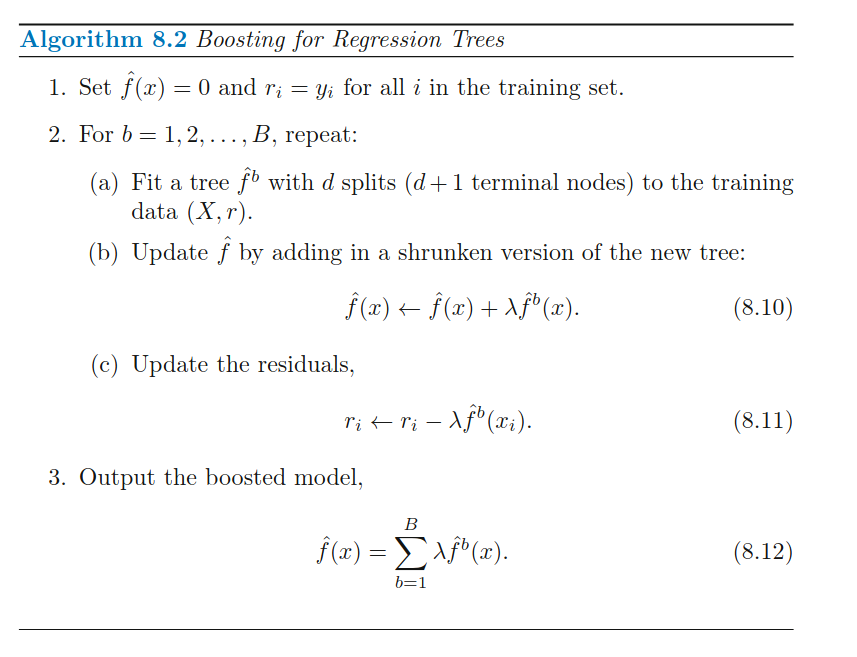
\includegraphics[width=\textwidth]{figs/boosting for regression trees.png}
    
\end{frame}

\begin{frame}{Boosting - Sammanfattninig}
    
    Finns många andra varianter:
    \begin{itemize}
        \item Gradient boosting:
        \begin{itemize}
            \item XGboost
            \item LightGBM
            \item CatBoost
        \end{itemize}
        \item Presterar bra och vinner ofta tävlingar.
    \end{itemize}

    Om vi jämför med baggning kan vi se:

    \begin{tabular}{l | l}
        Bagging & Boosting \\ \hline
        Kan träna modeller parallellt & Tränar modeller sekventiellt \\
        Använder bootstrappade dataset & Använder viktade dataset \\
        Överanpassar inte med ökande $B$ & Kan överanpassa när $B$ ökar \\
        Minskar variansen men inte bias & Minska varians och bias.
        
    \end{tabular}

\end{frame}

\end{document}